\section{The \name{}}
\label{sec:nanoPU}
The \name{} is a new domain-specific processor optimized for running nanotasks---with low average and tail latency---for compute-intensive distributed applications based on nanoservices. 
A \name{} consists of one or more CPU cores and one or more low-latency NICs. 
The CPU cores are slightly modified cores; our design is based on the popular, open-source RISC-V ISA~\cite{riscv}. 
The low-latency NIC is inspired by the recently proposed {\em Lightning NIC (L-NIC)}~\cite{lnic}, a novel approach that terminates the transport layer in hardware, then delivers message data right into the registers at the heart of the CPU core.  
The L-NIC approach minimizes latency (and unpredictability) by bypassing DMA, cache, and DRAM entirely. 
Our \name{} design also adds a novel hardware thread scheduler, to minimize the time (and variability) from when a message arrives until the thread starts processing it.

Figure~\ref{fig:nanoPU} shows a high-level block diagram of a \name{}. 
This particular example shows one network interface shared by three cores, but in general the \name{} is designed to work with any ratio of NICs to cores. 
Depending on the need, it may make sense to build \name{}s with one core per NIC (\eg, for small embedded systems), all the way to hundreds of cores per NIC. 
For example, it would be practical today to design a chip with 500 cores~\cite{celerity, kilocore} and over a hundred \SI{100}{Gb/s} Ethernet interfaces;\footnote{Commercial switch chips exist with $128\times 100$ Gb/s Ethernet MACs today.} in this example, the ratio would be five cores per NIC. 
Of course, many other ratios are possible and the ideal ratio depends on the application, technology, and economics. 

\begin{figure}
  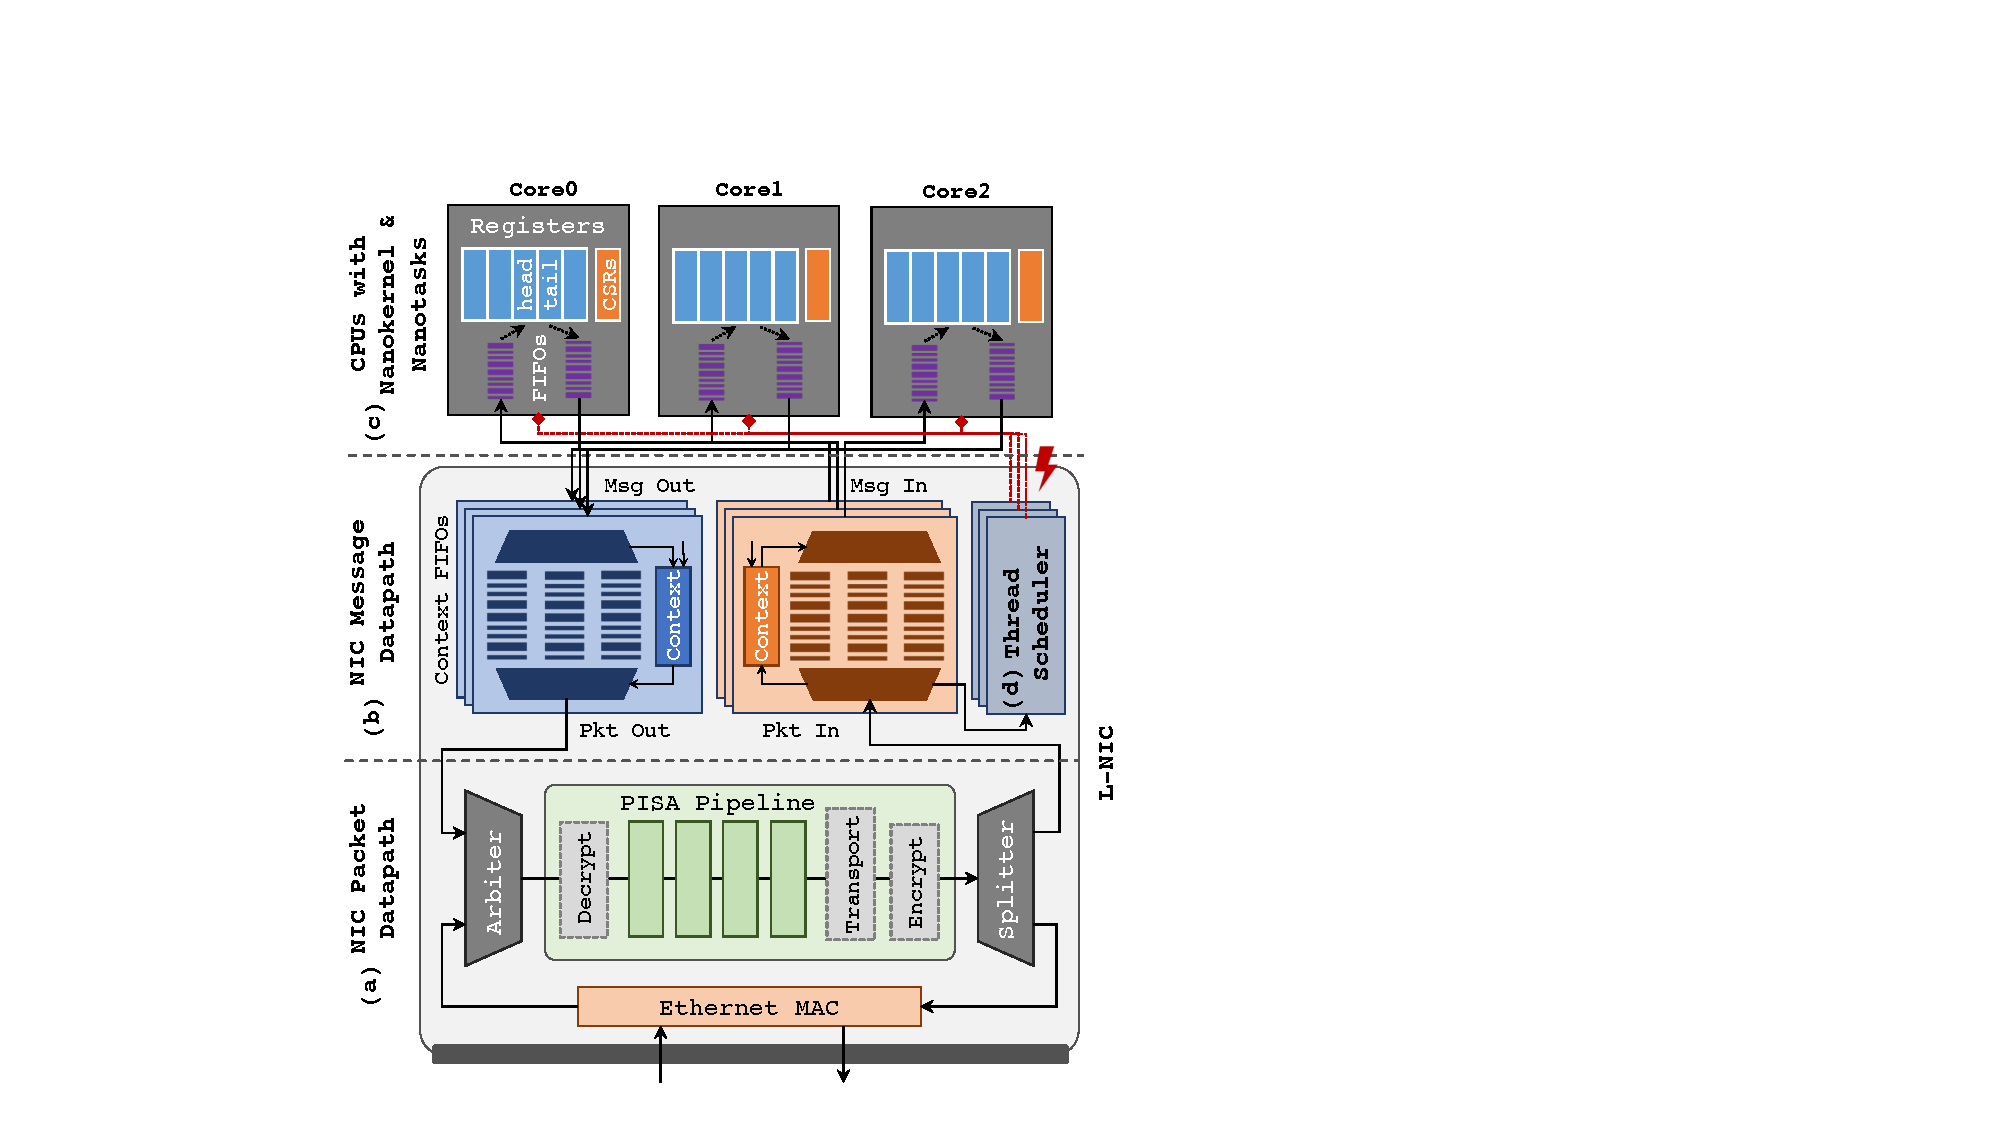
\includegraphics[width=0.95\linewidth]{./figures/nanopu-arch}
  \caption{The \name{} architecture. The NIC includes an event-driven PISA pipeline, and provides an RPC message abstraction to a thread via dedicated RX/TX registers in the CPU. CPU cores run a nanokernel and user nanotasks.}
  \label{fig:nanoPU}
\end{figure}

The \name{} is a domain-specific processor. 
With Moore's Law slowing down, new domain-specific processors are being widely used as accelerators for specific, high-volume workloads, such as graphics~\cite{nvidia-geforce}, machine learning~\cite{tensorflow} and networking~\cite{RMT}. 
While the \name{} is not nearly as radical a departure from a general-purpose CPU as, say, a GPU, TPU or programmable switch (after all, our design relies heavily on an existing core), the \name{} shares the approach of tailoring the chip design for a specific class of applications.\footnote{As an aside, it is only possible to consider prototyping a \name{} in a university because of two recent trends: RISC-V provides a remarkably stable starting point, and the narrow performance gap between the leading edge process (currently \SI{7}{nm}) and the closest already-paid-for process (\SI{16}{nm}) makes it economically feasible to build an interesting \name{}.}

If \name{} is so fast, why are not all CPUs designed this way? 
It is because general-purpose CPUs are optimized for general-purpose workloads, most of which are memory-intensive. 
They are ``load-store'' machines, with memory as a first-class citizen. 
Arriving and departing packet data must pass through the memory subsystem first, on its way in and out of the CPU. 
General-purpose CPUs put memory in the network and attach compute to memory, which makes perfect sense for memory-intensive applications.
Our approach is, instead, to make network messages first-class citizens in their own right, independent of memory. 
Network messages arrive directly into the CPU, without needing to make their way through the memory hierarchy. 
The \name{} is designed to tightly couple compute directly to the network, and then attach memory on the side as needed.

The \name{} has the following key characteristics that we visit, in turn, in the next few subsections: 
\begin{itemize}[topsep=0.4\baselineskip, leftmargin=20pt]
    \item {\bf NIC Packet Datapath:} A programmable event-driven PISA "match action unit" (MAU) pipeline~\cite{event-driven-pisa} on the NIC to process packet headers as they arrive and depart, terminate tunnels, encrypt/decrypt and compress/decompress data; and a low-latency transport protocol in hardware, such as Homa~\cite{homa} or NDP~\cite{ndp}.
    
    \item {\bf NIC Message Datapath:} A very low latency path---just a few clock cycles---from the network right to the very heart of the CPU core---its register file. 
    This reduces latency by 1--2 orders of magnitude; we do not believe there is a lower latency path to a running thread.
    
    \item {\bf Hardware Thread Scheduling:} In addition to moving network messages into the CPU quickly, the \name{} must also make sure that the appropriate application thread is running on the core so that it can start processing messages promptly. For this, \name{} includes a very low-latency, thread scheduler on the NIC and a light-weight nanokernel on the CPU.
\end{itemize}

These characteristics together enable the \name{} to process RPCs quickly and predictably, making it ideal for building compute-intensive, distributed applications.

\subsection{The NIC Datapath}
\label{ssec:nic-datapath}
The NIC datapath processes packets as they enter and leave the network.
Figure~\ref{fig:nanoPU} shows a high-level block diagram of the NIC packet-processing datapath.

The centerpiece of the NIC datapath is an event-driven PISA pipeline~\cite{event-driven-pisa}. 
The original PISA architecture, proposed in the RMT chip~\cite{RMT} and later used by Tofino~\cite{tofino}, is designed for mostly-stateless match-action processing of packet headers; for example for lookups, encapsulation, tunnels and telemetry.
Basic PISA only supports one type of event: the arrival of new packets. 
{\em Event-driven} PISA enhances the basic model to support other event types, such as packet drops, timers and state-dependent events. 
Section~\ref{ssec:nic-transport} describes how an event-driven PISA pipeline can directly support transport protocols in hardware, thus offloading per-packet processing from the CPU. 

The PISA pipeline also performs protocol processing: depending on the loaded P4~\cite{P4} program, it might add and remove Ethernet, IP, VXLAN, GRE, INT~\cite{INT} and transport headers. 
We also program it to add or remove a small per-context header containing the source IP address, a context ID, and message length~\Cref{fig:app-headers}.

\begin{figure}
 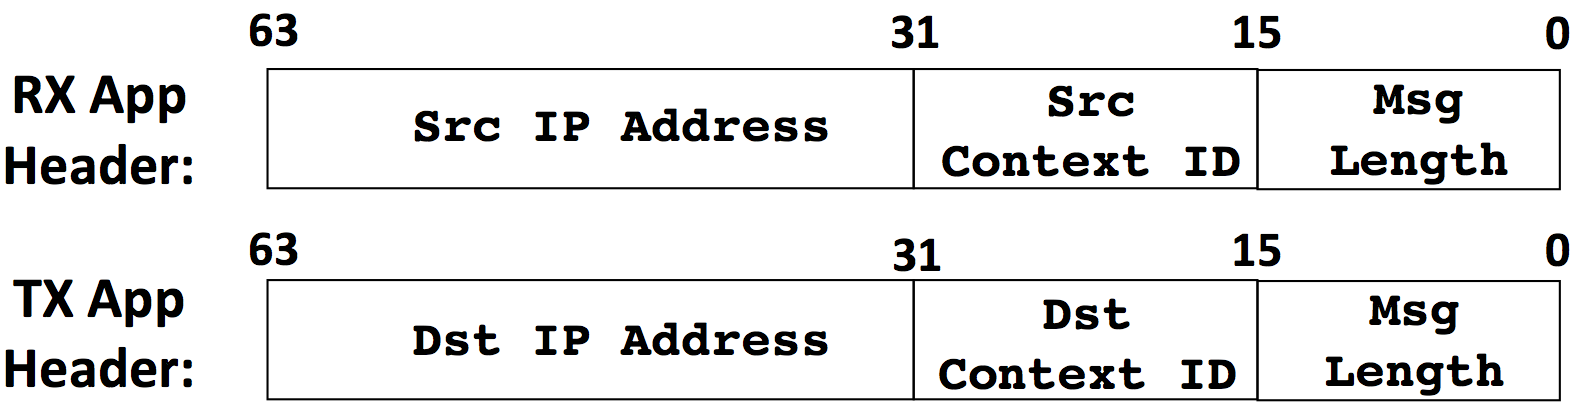
\includegraphics[width=\linewidth]{./figures/app-headers}
 \caption{Application header formats used in the NIC-Core interface.}
 \label{fig:app-headers}
\end{figure}

As others have noted, a P4-programmable PISA pipeline can also be used to accelerate some applications by offloading processing from the CPU (\eg, memory and disk caches~\cite{netcache}, load-balancers~\cite{silkroad}, consensus protocols~\cite{netchain} and firewalls~\cite{p4-firewall}). 
The L-NIC paper~\cite{lnic} describes how a PISA pipeline can accelerate nanoservices to search the Othello state-space.

\subsection{The NIC-Core Interface}
\label{ssec:niccore-interface}
The \name{}'s NIC Message Reassembler and Packetizer, shown in Figure~\ref{fig:nanoPU}, is responsible for assembling arriving packets into a self-contained RPC message, and then queuing the message into its destination nanotask's FIFO, where the message will remain until that nanotask's thread is scheduled. The message then flows, one word at a time, into the core's head register as the nanotask application processes the words. In the egress direction, the Message Reassembler and Packetizer breaks messages into packets before being sending them to the NIC Datapath.

We make two small modifications to allow the CPU core to interface with this layer of the NIC:
\begin{itemize}
    \item Two former general purpose registers (GPRs) are now reserved for a special purpose: one is the HEAD of the network receive queue, and the other is the TAIL of the network transmit queue. Applications must be compiled to avoid using reserved GPRs for temporary storage. Fortunately, \texttt{gcc} makes it easy to restrict register allocation via command line options.
    \item New control status registers (CSRs) are added for out-of-band communication between the CPU and the NIC. These are used to pass nanotask thread IDs and NIC-driven scheduling information between the NIC and the CPU. 
\end{itemize}

The NIC Message Reassembler and Packetizer hardware maintains transmit and receive FIFOs for each nanotask context (i.e. thread) that is currently pinned to the core. The hardware makes sure that the currently running thread only sees (i.e. reads from and writes to) its own per-context FIFO via the HEAD and TAIL GPRs.

The NIC exposes a {\em message} interface to applications running on the core, instead of a more traditional packet interface.
As a result, the \name{} NIC hardware must be responsible for the termination of the transport layer, including breaking messages into packets, ensuring reliable delivery, and processing message reassembly.

To convey relevant transport information, all messages sent or received by an application carry an 8-byte application header whose format is shown in Figure~\ref{fig:app-headers}. Applications must write the message's destination IP address, destination nanotask context ID and message length at the start of all outgoing messages. (Including the message length allows the NIC to determine when the application has finished writing a complete message.) Similarly, all incoming messages read by any application will begin with the message's source IP address, source nanotask context ID, and message length.

% \begin{figure}
%   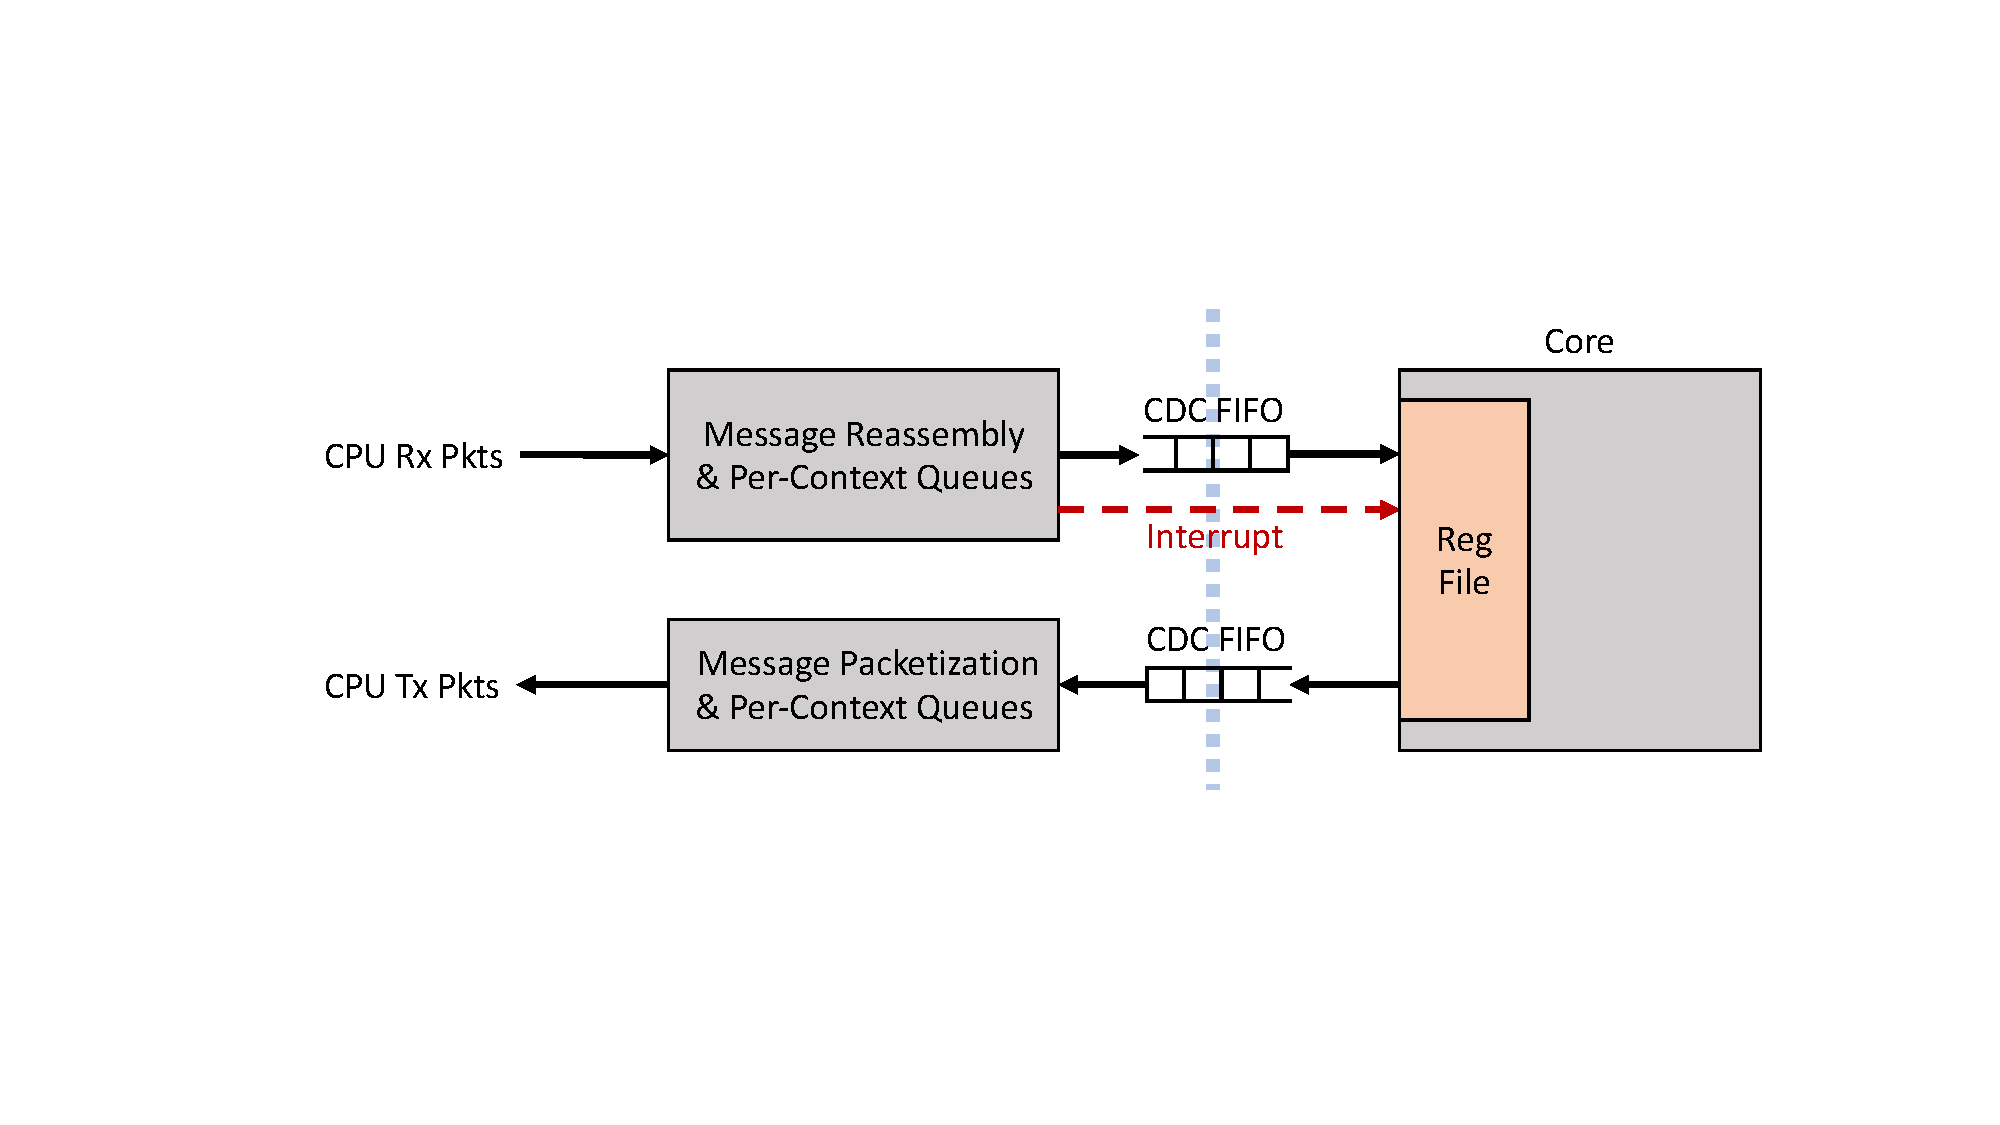
\includegraphics[width=\linewidth]{./figures/NIC-Core-Interface}
%   \caption{Block diagram of the \name{}'s NIC-Core interface.}
%   \label{fig:NIC-Core-Interface}
% \end{figure}

{\lstinputlisting[language=riscv]{code/loopback.S}
\vspace{-20pt}
\captionof{lstlisting}{Loopback with increment: A simple RISC-V \name{} assembly program to register a context \& priority with the NIC, wait for a 16B message to arrive then increment values during loopback from HEAD to TAIL FIFOs..}
\label{lst:asm}}

%\lstinputlisting[caption={Loopback with increment: A simple RISC-V \name{} assembly program to register a context \& priority with the NIC, wait for a 16B message to arrive then increment values during loopback from HEAD to TAIL FIFOs.}, label={lst:asm}]{code/loopback.S}

To illustrate how a \name{} interacts with its NIC, Listing~\ref{lst:asm} shows a simple loopback$+$increment program in RISC-V assembly language.  The program continuously reads 16 byte messages (consisting of two 8 byte integers) from the network, increments the integers, and sends the messages back to their sender. The program is described in more detail below.

The \textbf{\texttt{entry}} procedure registers a nanotask context ID with the NIC using the \texttt{lcurcontext} CSR (in the example, it sets the context ID to be 0). The procedure also sets the priority of the context (again to 0, the most urgent) using the  \texttt{lcurpriority} CSR. It then executes the command by setting the \texttt{lniccmd} CSR to value 1. \texttt{lniccmd} is a bit vector used by supervisor mode software to send commands to the NIC--in this case, it is used to tell the NIC to allocate an RX and a TX queue for context ID$=0$ with priority level$=0$. The \texttt{lniccmd} CSR can also be used to remove context IDs or to update the priority level.\footnote{Although the \texttt{lcurcontext}, \texttt{lcurpriority} and \texttt{lniccmd} CSRs convey hardware commands, they serve a similar purpose to opening or closing a socket in a traditional operating system.}

The \textbf{\texttt{wait\_msg}} procedure waits for a message to arrive in the RX queue by polling the \texttt{lmsgsrdy} CSR until it is set by the NIC, indicating that the context has messages to process. While it is waiting, the application tells the NIC that it is idle by setting the \texttt{lidle} CSR during the polling loop. The NIC thread scheduler uses the idle signal to evict waiting threads and, instead, schedule a new thread with a new message waiting to be processed. 

The \textbf{\texttt{loopback\_plus1\_16B}} procedure simply swaps the source and destination addresses by moving the application header (the first word of every message) from the head register (\texttt{t5}) to the tail register (\texttt{t6}), shown on line 20. It then increments every integer in the received message, appends them to the message being transmitted, and waits for the next message to arrive.

Applications that use variable length messages can use the message length (in the application header) to read the correct number of words from the network RX queue. If an application reads an empty RX queue, the resulting behavior is undefined - similar to reading an uninitialized variable.
\subsection{NIC-Driven Thread Scheduling}
\label{ssec:thread-scheduler}
In some specialized applications, thread scheduling might not be needed: Big HPC applications, for example, might pin every nanotask to a dedicated core for the duration of a run.
But this would not work for a cloud provider who needs more economical sharing of \name{}s by multiple nanoservice applications.
Nanotask threads will therefore need to be switched in and out frequently, and context switches must be extremely fast, else we will lose all the low latency benefits of nanoservices.

If \name{} relied on software scheduling it would be too slow. 
The fastest best-of-breed software schedulers use 5$\mu$s timer interrupts~\cite{shinjuku, shenango} which are much too slow for our $<1\mu$s nanotasks.
And so, instead, the \name{} decides which thread to run next in hardware on the NIC (\Cref{fig:nanoPU}d), then tells the CPU core. 
The NIC keeps track of the highest-priority nanotask with messages to process and interrupts the CPU to initiate a context switch under two conditions:

\begin{enumerate}
    \item A message arrives for a higher priority context than the one currently running on the core.
    \item The current context tells the NIC it is idle, and the NIC has messages for another context to process. 
    This condition prevents an idle high-priority context from starving a low-priority context with messages waiting to be processed.
\end{enumerate}

\Cref{fig:nic-scheduler} shows what happens when a message arrives for a higher-priority context than the one currently running on the core. 
In step \ballnumber{a}, the arriving message is enqueued into the RX queue for the high-priority context.
In step \ballnumber{b}, the thread scheduler tells the CPU that a high-priority message is waiting by updating the \verb|ltargetcontext| CSR and firing an interrupt.
The interrupt causes a trap into the nanokernel, which then reads the \verb|ltargetcontext| CSR and performs a switch to the high-priority context in step \ballnumber{c}, updating the \verb|lcurcontext| CSR.
At this point, the high-priority context is running on the core and is able to process the message in its RX queue.
When the high-priority context finishes processing the message, it tells the NIC that it is now idle by writing to a dedicated CSR called \verb|lidle|.
The NIC then initiates a context switch back to the low-priority context because it still has messages to process.

\shahbaz{will update Figure~\ref{fig:nic-scheduler} to contain the relevant CSRs}

\begin{figure}
  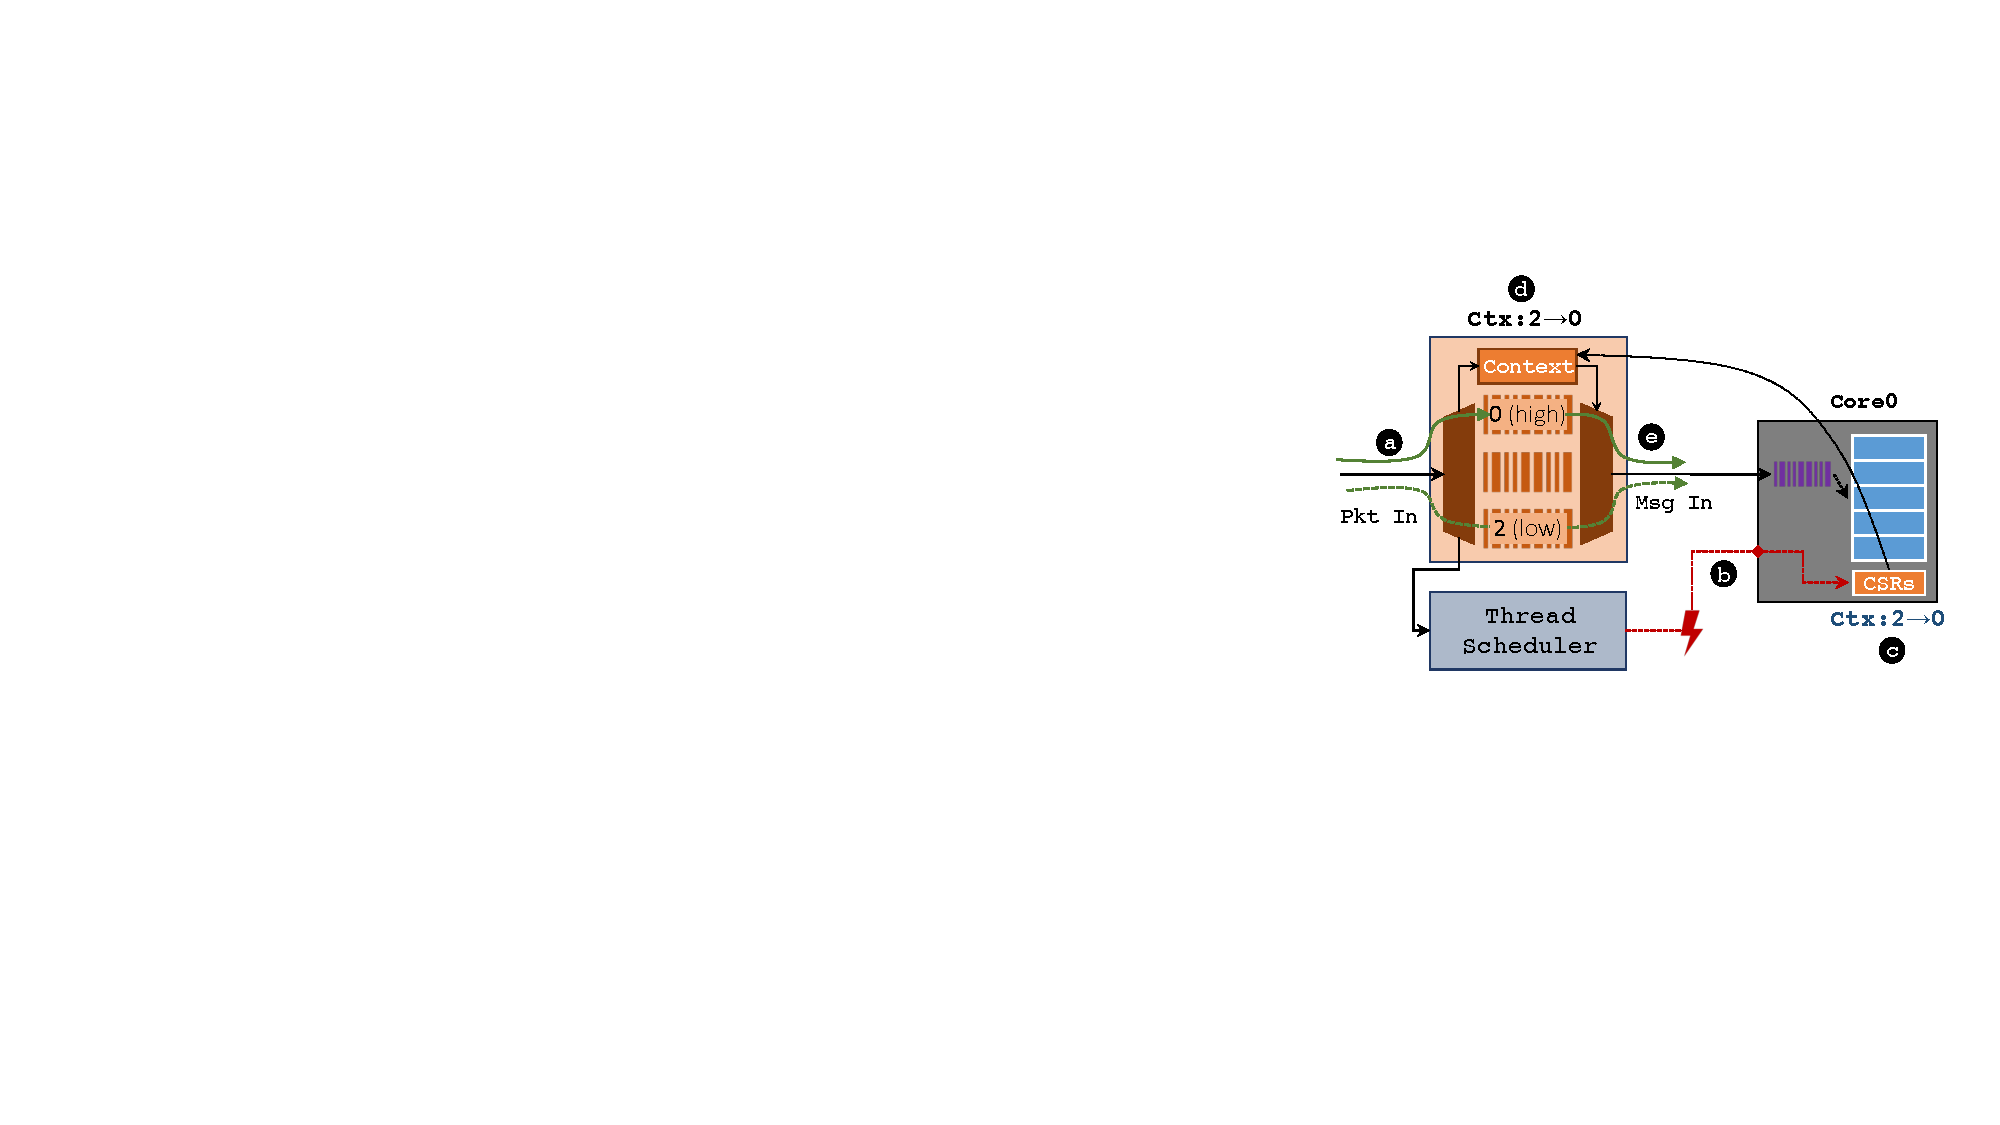
\includegraphics[width=0.8\linewidth]{./figures/thread-sched}
  \caption{The steps that occur when a low-priority thread running on a core is preempted by a higher-priority context.}
  \label{fig:nic-scheduler}
\end{figure}
\subsection{Terminating Transport in the NIC}
\label{ssec:nic-transport}
If the \name{} is to meet our aggressive latency target of $<1\mu$s from when an RPC message arrives over Ethernet until a response is sent back out, there is clearly no time to run a traditional transport networking stack in software. Therefore, \name{} runs a low-latency transport protocol in hardware, in the NIC, with support from the NIC's programmable pipeline. Note that transport protocols for low-latency applications (e.g., DCQCN for RDMA) are already fully implemented in hardware~\cite{cvl,connectx6} on state-of-the-art high-speed NICs available in today's market, vouching for the feasibility of a fully-offloaded transport protocol running in hardware.

We, however, don't mandate a specific transport protocol in this paper because we seem to be entering an era when different cloud providers prefer different transport protocols~\cite{timely,hpcc,dcqcn}. Instead we aim to provide some choices, within our tight latency budget.

The NIC therefore places minimal constraints on the transport protocol, while providing programmable hardware blocks to allow some choice by the network owner. We assume that the transport layer provides a reliable message abstraction to each thread, as well as network congestion control. It therefore must handle retransmissions and decide when packets should be sent. To guide our design, we assume it must be possible for the NIC to be programmed to implemented Homa~\cite{homa} and NDP~\cite{ndp}. Between them, they mandate most of the building blocks we need, including reliable transmission, immediate startup rate, receiver driven scheduling, a message abstraction to the CPU, and data-trimming (in the switches).

We observe that realizing a transport protocol in hardware requires the following functions in the programmable pipeline of a NIC.

\begin{itemize}
    \item Timers and timer-based event processing logic to realize various timer-based state transitions, such as retransmissions and timeouts.
    \item Pacers to rate-limit individual flows.
    \item Flow state machine to maintain per-flow state, including current rate or congestion-window size, sequence and acknowledgment numbers, connection-establishment status, counters, etc.
    \item Packetization/retransmission buffer to break a message into packets and hold packets until they are acknowledged by a receiver.
    \item Reordering buffer to handle out-of-order delivery of packets.
    \item Packet generators to realize receiver-driven transport protocols that keep generating credit packets for senders.
\end{itemize}

The event-driven PISA pipeline~\cite{event-driven-pisa} already provides most of the mechanisms we need for sophisticated stateful operations (\eg, state machines, timer events and packet generation), and can be extended to add support for message reassembly and retransmit buffers~\cite{schuehler2004modular, intel-rapidio}. Because nanoservice messages sizes will be very small, the amount of SRAM needed to realize these buffers will be sufficiently small for a cost- and power-efficient hardware implementation. With these mechanisms, we believe the \name{} can run a complete transport stack on the NIC with very low latency. While we have a design for each of these building blocks, we will explain the details of those in our follow-on paper.

\iffalse
The key components that enable the NIC to terminate a transport protocol are described below.

The \textbf{event-driven PISA pipeline~\cite{event-driven-pisa}} is a programmable data-plane architecture that enables us to write programs that process data-plane events in the background of data packet processing, that is, without affecting the rate at which data packets are processed.
It does this by scheduling and aggregating memory accesses.
This mechanism helps to enable transport logic processing which must perform more sophisticated stateful operations than basic packet forwarding.

The \textbf{timer event generation module} is a hardware mechanism within the aforementioned event-driven PISA pipeline that is able to maintain $N$ timers (e.g. one per active message or one per active RPC).
The timer module supports the following three operations per-timer:
\begin{itemize}
    \item Schedule - add a new timer
    \item Reschedule - restart an existing timer
    \item Cancel - remove the state associated with an existing timer
\end{itemize}
These timer events are processed in the background of data packet processing and are used to determine when a data packet retransmission must be sent or when a message (or RPC) has expired and its state must be cleaned up.

The \textbf{programmable packet generation module} is used to generate acknowledgement and/or message completion packets.

The \textbf{packetization buffer} stores messages sent from the CPU and generates packets that are subsequently processed by the event-driven PISA pipeline before being transmitted.
It also supports retransmitting data packets within a message when a packet drop is detected.

The \textbf{message reassembly buffer} is able to reassemble potentially multi-packet messages with duplicate packets into a single message that is then delivered to the appropriate RX queue for the destination context.
\fi
